\PassOptionsToPackage{unicode=true}{hyperref} % options for packages loaded elsewhere
\PassOptionsToPackage{hyphens}{url}
%
\documentclass[]{article}
\usepackage{lmodern}
\usepackage{amssymb,amsmath}
\usepackage{ifxetex,ifluatex}
\usepackage{fixltx2e} % provides \textsubscript
\ifnum 0\ifxetex 1\fi\ifluatex 1\fi=0 % if pdftex
  \usepackage[T1]{fontenc}
  \usepackage[utf8]{inputenc}
  \usepackage{textcomp} % provides euro and other symbols
\else % if luatex or xelatex
  \usepackage{unicode-math}
  \defaultfontfeatures{Ligatures=TeX,Scale=MatchLowercase}
\fi
% use upquote if available, for straight quotes in verbatim environments
\IfFileExists{upquote.sty}{\usepackage{upquote}}{}
% use microtype if available
\IfFileExists{microtype.sty}{%
\usepackage[]{microtype}
\UseMicrotypeSet[protrusion]{basicmath} % disable protrusion for tt fonts
}{}
\IfFileExists{parskip.sty}{%
\usepackage{parskip}
}{% else
\setlength{\parindent}{0pt}
\setlength{\parskip}{6pt plus 2pt minus 1pt}
}
\usepackage{hyperref}
\hypersetup{
            pdfborder={0 0 0},
            breaklinks=true}
\urlstyle{same}  % don't use monospace font for urls
\usepackage{color}
\usepackage{fancyvrb}
\newcommand{\VerbBar}{|}
\newcommand{\VERB}{\Verb[commandchars=\\\{\}]}
\DefineVerbatimEnvironment{Highlighting}{Verbatim}{commandchars=\\\{\}}
% Add ',fontsize=\small' for more characters per line
\newenvironment{Shaded}{}{}
\newcommand{\AlertTok}[1]{\textcolor[rgb]{1.00,0.00,0.00}{\textbf{#1}}}
\newcommand{\AnnotationTok}[1]{\textcolor[rgb]{0.38,0.63,0.69}{\textbf{\textit{#1}}}}
\newcommand{\AttributeTok}[1]{\textcolor[rgb]{0.49,0.56,0.16}{#1}}
\newcommand{\BaseNTok}[1]{\textcolor[rgb]{0.25,0.63,0.44}{#1}}
\newcommand{\BuiltInTok}[1]{#1}
\newcommand{\CharTok}[1]{\textcolor[rgb]{0.25,0.44,0.63}{#1}}
\newcommand{\CommentTok}[1]{\textcolor[rgb]{0.38,0.63,0.69}{\textit{#1}}}
\newcommand{\CommentVarTok}[1]{\textcolor[rgb]{0.38,0.63,0.69}{\textbf{\textit{#1}}}}
\newcommand{\ConstantTok}[1]{\textcolor[rgb]{0.53,0.00,0.00}{#1}}
\newcommand{\ControlFlowTok}[1]{\textcolor[rgb]{0.00,0.44,0.13}{\textbf{#1}}}
\newcommand{\DataTypeTok}[1]{\textcolor[rgb]{0.56,0.13,0.00}{#1}}
\newcommand{\DecValTok}[1]{\textcolor[rgb]{0.25,0.63,0.44}{#1}}
\newcommand{\DocumentationTok}[1]{\textcolor[rgb]{0.73,0.13,0.13}{\textit{#1}}}
\newcommand{\ErrorTok}[1]{\textcolor[rgb]{1.00,0.00,0.00}{\textbf{#1}}}
\newcommand{\ExtensionTok}[1]{#1}
\newcommand{\FloatTok}[1]{\textcolor[rgb]{0.25,0.63,0.44}{#1}}
\newcommand{\FunctionTok}[1]{\textcolor[rgb]{0.02,0.16,0.49}{#1}}
\newcommand{\ImportTok}[1]{#1}
\newcommand{\InformationTok}[1]{\textcolor[rgb]{0.38,0.63,0.69}{\textbf{\textit{#1}}}}
\newcommand{\KeywordTok}[1]{\textcolor[rgb]{0.00,0.44,0.13}{\textbf{#1}}}
\newcommand{\NormalTok}[1]{#1}
\newcommand{\OperatorTok}[1]{\textcolor[rgb]{0.40,0.40,0.40}{#1}}
\newcommand{\OtherTok}[1]{\textcolor[rgb]{0.00,0.44,0.13}{#1}}
\newcommand{\PreprocessorTok}[1]{\textcolor[rgb]{0.74,0.48,0.00}{#1}}
\newcommand{\RegionMarkerTok}[1]{#1}
\newcommand{\SpecialCharTok}[1]{\textcolor[rgb]{0.25,0.44,0.63}{#1}}
\newcommand{\SpecialStringTok}[1]{\textcolor[rgb]{0.73,0.40,0.53}{#1}}
\newcommand{\StringTok}[1]{\textcolor[rgb]{0.25,0.44,0.63}{#1}}
\newcommand{\VariableTok}[1]{\textcolor[rgb]{0.10,0.09,0.49}{#1}}
\newcommand{\VerbatimStringTok}[1]{\textcolor[rgb]{0.25,0.44,0.63}{#1}}
\newcommand{\WarningTok}[1]{\textcolor[rgb]{0.38,0.63,0.69}{\textbf{\textit{#1}}}}
\usepackage{graphicx,grffile}
\makeatletter
\def\maxwidth{\ifdim\Gin@nat@width>\linewidth\linewidth\else\Gin@nat@width\fi}
\def\maxheight{\ifdim\Gin@nat@height>\textheight\textheight\else\Gin@nat@height\fi}
\makeatother
% Scale images if necessary, so that they will not overflow the page
% margins by default, and it is still possible to overwrite the defaults
% using explicit options in \includegraphics[width, height, ...]{}
\setkeys{Gin}{width=\maxwidth,height=\maxheight,keepaspectratio}
\setlength{\emergencystretch}{3em}  % prevent overfull lines
\providecommand{\tightlist}{%
  \setlength{\itemsep}{0pt}\setlength{\parskip}{0pt}}
\setcounter{secnumdepth}{0}
% Redefines (sub)paragraphs to behave more like sections
\ifx\paragraph\undefined\else
\let\oldparagraph\paragraph
\renewcommand{\paragraph}[1]{\oldparagraph{#1}\mbox{}}
\fi
\ifx\subparagraph\undefined\else
\let\oldsubparagraph\subparagraph
\renewcommand{\subparagraph}[1]{\oldsubparagraph{#1}\mbox{}}
\fi

% set default figure placement to htbp
\makeatletter
\def\fps@figure{htbp}
\makeatother


\date{}

\begin{document}

\hypertarget{projecte-asix-2k22}{%
\section{\texorpdfstring{\textbf{Projecte ASIX
2k22}}{Projecte ASIX 2k22}}\label{projecte-asix-2k22}}

\hypertarget{escola-del-treball}{%
\subsection{\texorpdfstring{\textbf{Escola Del
Treball}}{Escola Del Treball}}\label{escola-del-treball}}

\hypertarget{hisx-2021-2022}{%
\subsubsection{\texorpdfstring{\textbf{2HISX
2021-2022}}{2HISX 2021-2022}}\label{hisx-2021-2022}}

\hypertarget{aaron-andal-cristian-condolo}{%
\subsubsection{\texorpdfstring{\textbf{Aaron Andal \& Cristian
Condolo}}{Aaron Andal \& Cristian Condolo}}\label{aaron-andal-cristian-condolo}}

\hypertarget{cryptosec-careful-where-you-step-in}{%
\section{\texorpdfstring{\textbf{CryptoSEC}: ``\emph{Careful where you
step
in}''}{CryptoSEC: ``Careful where you step in''}}\label{cryptosec-careful-where-you-step-in}}

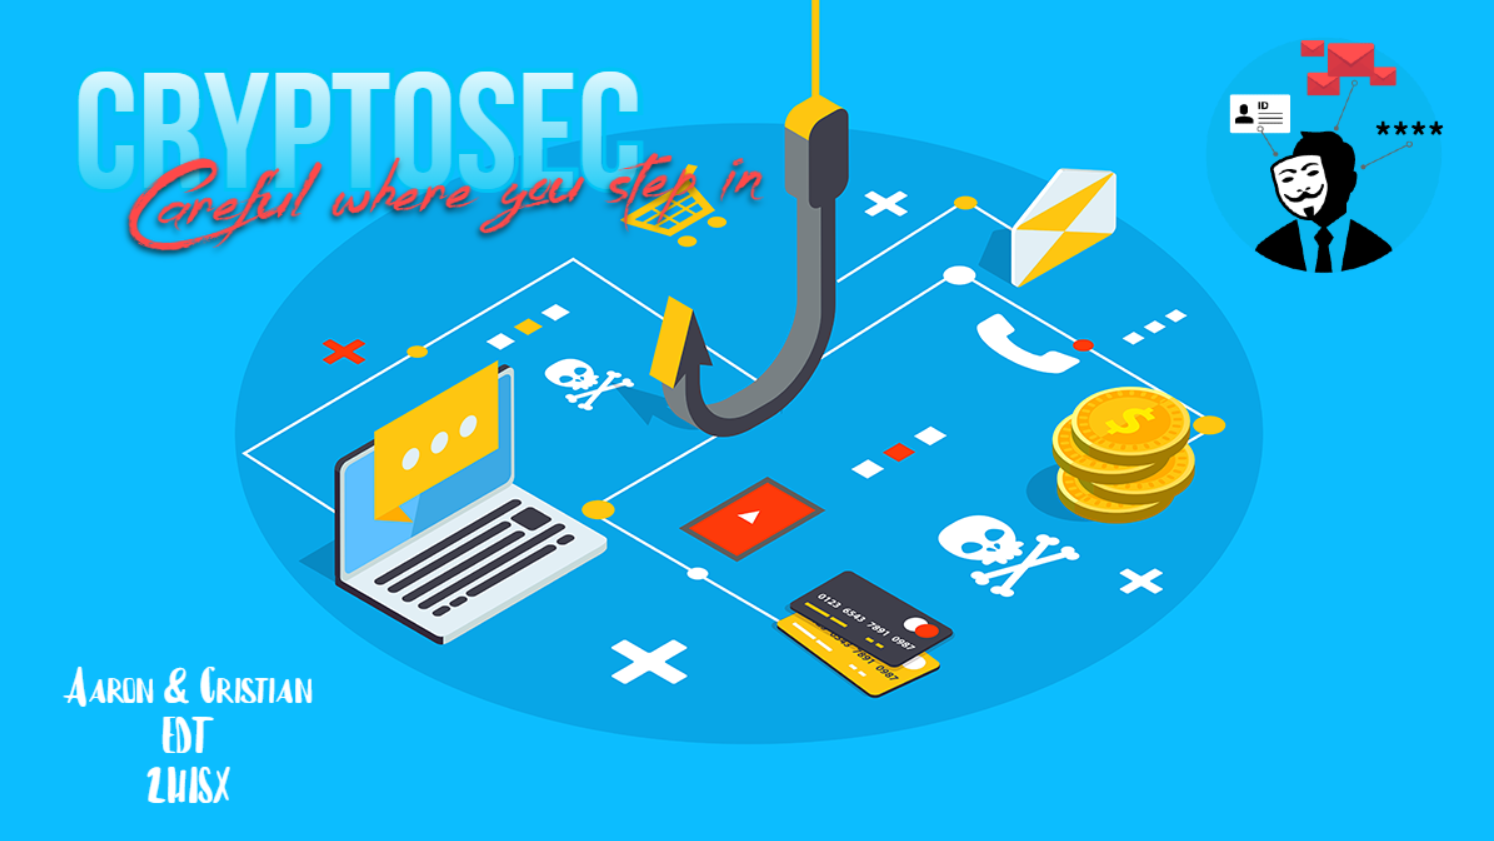
\includegraphics{./tex2pdf.-702480177ac5f5f6/785b57206d80bd3d5ef15f036481e103db8435a1.png}
\textgreater{} \textbf{Img Source}: \emph{@Aaron \& @Cristian 's GitHub}

\hypertarget{index}{%
\section{\texorpdfstring{\textbf{Index}}{Index}}\label{index}}

\begin{itemize}
\item
  \textbf{Apache2}: \protect\hyperlink{apache2}{--\textgreater{} readME
  \textless{}--}
\item
  \textbf{Avantatges}: \protect\hyperlink{avantatges}{--\textgreater{}
  readME \textless{}--}
\item
  \textbf{Desavantatges}:
  \protect\hyperlink{desavantatges}{--\textgreater{} readME
  \textless{}--}
\item
  \textbf{Instal·lació Apache2 per a SOA CryptoSEC}:
  \protect\hyperlink{installaciuxf3-apache2-per-a-soa-cryptosec}{--\textgreater{}
  readME \textless{}--}
\item
  \textbf{Configurar Hosts Virtuals}:
  \protect\hyperlink{configurar-hosts-virtuals}{--\textgreater{} readME
  \textless{}--}
\item
  \textbf{OpenSSL}: \protect\hyperlink{openssl}{--\textgreater{} readME
  \textless{}--}

  \begin{itemize}
  \item
    \textbf{Creació de claus i certificats}:
    \protect\hyperlink{creaciuxf3-de-claus-i-certificats}{--\textgreater{}
    readME \textless{}--}
  \item
    \textbf{CA Veritat Absoluta}:
    \protect\hyperlink{ca-veritat-absoluta}{--\textgreater{} readME
    \textless{}--}
  \item
    \textbf{Habilitar SSL per HTTP}:
    \protect\hyperlink{habilitar-ssl-per-http}{--\textgreater{} readME
    \textless{}--}
  \end{itemize}
\item
  \textbf{Bibliografia}:
  \protect\hyperlink{bibliografia}{--\textgreater{} readME
  \textless{}--}
\end{itemize}

\hypertarget{apache2}{%
\section{\texorpdfstring{\textbf{Apache2}}{Apache2}}\label{apache2}}

Apache és un servidor web de codi obert, multiplataforma i gratuït.
Aquest web server és un dels més utilitzats al món, actualment el 43\%
dels llocs web funcionen amb ell.

\includegraphics{./tex2pdf.-702480177ac5f5f6/0b60666cafefc37299ce2a577add08d1c469d812.jpg}
\textgreater{} \textbf{Img Source}:
\emph{https://www.unfantasmaenelsistema.com/wp-content/uploads/2019/12/hd221.jpg}

Apache té una estructura basada en mòduls, que permet activar i
desactivar funcionalitats addicionals, per exemple, mòduls de seguretat
com mod\_security, mòduls de memòria cau com Varnish , o de
personalització de capçaleres com mod\_headers.

També permet ajustar els paràmetres de PHP del teu hosting de forma
personalitzada mitjançant el fitxer .htaccess .

\includegraphics{./tex2pdf.-702480177ac5f5f6/e67cf6c8f8c98bb8378f69c9b8d77879f492c412.png}
\textgreater{} \textbf{Img Source}:
\emph{https://www.webempresa.com/wp-content/uploads/2021/10/servidor-rueda-dentada-400.png}

\hypertarget{avantatges}{%
\subsection{\texorpdfstring{\textbf{Avantatges}}{Avantatges}}\label{avantatges}}

Els principals avantatges d'usar aquest servei web són els següents:

\begin{itemize}
\item
  De codi \emph{obert} i \textbf{gratuït}, amb una gran comunitat
  dusuaris.
\item
  Pegats de seguretat regulars i actualitzats amb freqüència.
\item
  Estructura basada en \textbf{mòduls}.
\item
  Multiplataforma. Està disponible a servidors \textbf{Windows} i
  \textbf{Linux}.
\item
  Personalització mitjançant \textbf{.htaccess} independent a cada
  hosting.
\item
  Compatible amb els principals \textbf{CMS} i \textbf{botigues online}
  i plataformes \textbf{e-learning}
\end{itemize}

\includegraphics{./tex2pdf.-702480177ac5f5f6/436e3a03e7e922c498bc3a27404979512c61d24e.png}
\textgreater{} \textbf{Img Source}:
\emph{https://www.webempresa.com/wp-content/uploads/2021/10/servidor-flecha-up-arriba-400.png}

\hypertarget{desavantatges}{%
\subsection{\texorpdfstring{\textbf{Desavantatges}}{Desavantatges}}\label{desavantatges}}

\begin{itemize}
\item
  Presenta problemes d'estabilitat per sobre de les 10.000 connexions
\item
  Un ús abusiu de mòduls poden generar bretxes de seguretat.
\end{itemize}

\includegraphics{./tex2pdf.-702480177ac5f5f6/cd2722593e4725de51e7282a21d0c0299c1a5d38.png}
\textgreater{} \textbf{Img Source}:
\emph{https://www.webempresa.com/wp-content/uploads/2021/10/servidor-flecha-down-abajo-400.png}

\hypertarget{installaciuxf3-apache2-per-a-soa-cryptosec}{%
\section{\texorpdfstring{\textbf{Instal·lació Apache2 per a SOA
CryptoSEC}}{Instal·lació Apache2 per a SOA CryptoSEC}}\label{installaciuxf3-apache2-per-a-soa-cryptosec}}

\begin{enumerate}
\def\labelenumi{\arabic{enumi}.}
\tightlist
\item
  Actualitzar el \textbf{repositori} i instal·lar \textbf{apache2}.
\end{enumerate}

\begin{Shaded}
\begin{Highlighting}[]
\FunctionTok{sudo}\NormalTok{ apt update}
\end{Highlighting}
\end{Shaded}

\begin{Shaded}
\begin{Highlighting}[]
\FunctionTok{sudo}\NormalTok{ apt install apache2}
\end{Highlighting}
\end{Shaded}

\begin{enumerate}
\def\labelenumi{\arabic{enumi}.}
\setcounter{enumi}{1}
\tightlist
\item
  Readjustar el firewall perque permeti Apache2. Apache es registra amb
  UFW per proporcionar alguns perfils d'aplicació que es poden utilitzar
  per habilitar o deshabilitar l'accés a Apache a través del
  \emph{firewall}.
\end{enumerate}

Llistem els perfils de \textbf{ufw}.

\begin{Shaded}
\begin{Highlighting}[]
\FunctionTok{sudo}\NormalTok{ ufw app list}
\end{Highlighting}
\end{Shaded}

Com ho indica el resultat, hi ha tres perfils disponibles per a Apache:

\begin{itemize}
\item
  \textbf{Apache}: aquest perfil obre només el port 80 (tràfic web
  normal no xifrat)
\item
  \textbf{Apache Full}: aquest perfil obre el port 80 (tràfic web normal
  no xifrat) i el port 443 (tràfic TLS/SSL xifrat)
\item
  \textbf{Apache Secure}: aquest perfil obre només el port 443 (tràfic
  TLS/SSL xifrat)
\end{itemize}

\begin{Shaded}
\begin{Highlighting}[]
\ExtensionTok{Output}
\ExtensionTok{Available}\NormalTok{ applications:}
  \ExtensionTok{Apache}
  \ExtensionTok{Apache}\NormalTok{ Full}
  \ExtensionTok{Apache}\NormalTok{ Secure}
  \ExtensionTok{OpenSSH}
\end{Highlighting}
\end{Shaded}

El resultat proporcionarà una llista del trànsit de HTTP que es permet:

\begin{Shaded}
\begin{Highlighting}[]
\FunctionTok{sudo}\NormalTok{ ufw allow }\StringTok{'Apache'}
\end{Highlighting}
\end{Shaded}

\begin{Shaded}
\begin{Highlighting}[]
\FunctionTok{sudo}\NormalTok{ ufw status}
\end{Highlighting}
\end{Shaded}

\begin{Shaded}
\begin{Highlighting}[]
\ExtensionTok{Output}
\ExtensionTok{Status}\NormalTok{: active}

\ExtensionTok{To}\NormalTok{                         Action      From}
\ExtensionTok{--}\NormalTok{                         ------      ----}
\ExtensionTok{OpenSSH}\NormalTok{                    ALLOW       Anywhere                  }
\ExtensionTok{Apache}\NormalTok{                     ALLOW       Anywhere                }
\ExtensionTok{OpenSSH}\NormalTok{ (v6)               }\ExtensionTok{ALLOW}\NormalTok{       Anywhere (v6)             }
\ExtensionTok{Apache}\NormalTok{ (v6)                }\ExtensionTok{ALLOW}\NormalTok{       Anywhere (v6)}
\end{Highlighting}
\end{Shaded}

\begin{enumerate}
\def\labelenumi{\arabic{enumi}.}
\setcounter{enumi}{2}
\tightlist
\item
  Comprovar el servidor web.
\end{enumerate}

\begin{Shaded}
\begin{Highlighting}[]
\FunctionTok{sudo}\NormalTok{ systemctl status apache2}
\end{Highlighting}
\end{Shaded}

\begin{Shaded}
\begin{Highlighting}[]
\ExtensionTok{Output}
\ExtensionTok{apache2.service}\NormalTok{ - The Apache HTTP Server}
     \ExtensionTok{Loaded}\NormalTok{: loaded (/lib/systemd/system/apache2.service}\KeywordTok{;} \ExtensionTok{enabled}\KeywordTok{;} \ExtensionTok{vendor}\NormalTok{ preset: enabled)}
     \ExtensionTok{Active}\NormalTok{: active (running) }\ExtensionTok{since}\NormalTok{ Thu 2020-04-23 22:36:30 UTC}\KeywordTok{;} \ExtensionTok{20h}\NormalTok{ ago}
       \ExtensionTok{Docs}\NormalTok{: https://httpd.apache.org/docs/2.4/}
   \ExtensionTok{Main}\NormalTok{ PID: 29435 (apache2)}
      \ExtensionTok{Tasks}\NormalTok{: 55 (limit: 1137)}
     \ExtensionTok{Memory}\NormalTok{: 8.0M}
     \ExtensionTok{CGroup}\NormalTok{: /system.slice/apache2.service}
\NormalTok{             ├─}\ExtensionTok{29435}\NormalTok{ /usr/sbin/apache2 -k start}
\NormalTok{             ├─}\ExtensionTok{29437}\NormalTok{ /usr/sbin/apache2 -k start}
\NormalTok{             └─}\ExtensionTok{29438}\NormalTok{ /usr/sbin/apache2 -k start}
\end{Highlighting}
\end{Shaded}

\begin{enumerate}
\def\labelenumi{\arabic{enumi}.}
\setcounter{enumi}{3}
\tightlist
\item
  Obrir un navegador i posar la IP del SOA 10.200.243.164. Per HTTP. Més
  tard configurarem HTTPS.
\end{enumerate}

\includegraphics{./tex2pdf.-702480177ac5f5f6/08c0074b7a37880aeb7edc0481f7a24621593036.png}
\textgreater{} \textbf{Img Source}:
\emph{https://assets.digitalocean.com/articles/how-to-install-lamp-ubuntu-16/small\_apache\_default.png}

\begin{enumerate}
\def\labelenumi{\arabic{enumi}.}
\setcounter{enumi}{4}
\tightlist
\item
  Administrar Apache2:
\end{enumerate}

Per aturar el vostre servidor web, escriviu el següent:

\begin{Shaded}
\begin{Highlighting}[]
\FunctionTok{sudo}\NormalTok{ systemctl stop apache2}
\end{Highlighting}
\end{Shaded}

Per iniciar el servidor web quan no estigui actiu, escriviu el següent:

\begin{Shaded}
\begin{Highlighting}[]
\FunctionTok{sudo}\NormalTok{ systemctl start apache2}
\end{Highlighting}
\end{Shaded}

Per aturar i després iniciar el servei de nou, escriviu el següent:

\begin{Shaded}
\begin{Highlighting}[]
\FunctionTok{sudo}\NormalTok{ systemctl restart apache2}
\end{Highlighting}
\end{Shaded}

Si només feu canvis de configuració, Apache sovint es pot recarregar
sense tancar connexions. Per fer-ho, utilitzeu aquesta ordre:

\begin{Shaded}
\begin{Highlighting}[]
\FunctionTok{sudo}\NormalTok{ systemctl reload apache2}
\end{Highlighting}
\end{Shaded}

Per defecte, Apache està configurat per iniciar automàticament quan el
servidor ho fa. Si no és el que voleu, deshabiliteu aquest comportament
escrivint el següent:

\begin{Shaded}
\begin{Highlighting}[]
\FunctionTok{sudo}\NormalTok{ systemctl disable apache2}
\end{Highlighting}
\end{Shaded}

Per tornar a habilitar el servei de manera que es carregui a l'inici,
escriviu el següent:

\begin{Shaded}
\begin{Highlighting}[]
\FunctionTok{sudo}\NormalTok{ systemctl enable apache2}
\end{Highlighting}
\end{Shaded}

\hypertarget{configurar-hosts-virtuals}{%
\section{\texorpdfstring{\textbf{Configurar hosts
virtuals}}{Configurar hosts virtuals}}\label{configurar-hosts-virtuals}}

En utilitzar el servidor web \textbf{Apache}, podeu utilitzar hosts
virtuals (similars a blocs de servidor de Nginx) per encapsular detalls
de configuració i allotjar més d'un domini des d'un únic servidor.

El nostre domini es \textbf{cryptosec.net}. És a dir quan l'usuari posi
\textbf{cryptosec.net} al navegador anirà a parar a la nostra pàgina web
que està allotjada en \textbf{/var/www/html/cryptosec/}.

\begin{enumerate}
\def\labelenumi{\arabic{enumi}.}
\tightlist
\item
  Crear el directori \textbf{cryptosec} a \textbf{/var/www/html}
\end{enumerate}

\begin{Shaded}
\begin{Highlighting}[]
\FunctionTok{sudo}\NormalTok{ mkdir /var/www/html/cryptosec}
\end{Highlighting}
\end{Shaded}

\begin{enumerate}
\def\labelenumi{\arabic{enumi}.}
\setcounter{enumi}{1}
\tightlist
\item
  Cambiem el owner.
\end{enumerate}

\begin{Shaded}
\begin{Highlighting}[]
\FunctionTok{sudo}\NormalTok{ chown -R }\VariableTok{$USER}\NormalTok{:}\VariableTok{$USER}\NormalTok{ /var/www/html/cryptosec}
\end{Highlighting}
\end{Shaded}

\begin{enumerate}
\def\labelenumi{\arabic{enumi}.}
\setcounter{enumi}{2}
\tightlist
\item
  Els permisos dels roots web haurien de ser correctes si no vau
  modificar el valor umask, que estableix permisos de fitxers
  predeterminats.
\end{enumerate}

\begin{Shaded}
\begin{Highlighting}[]
\FunctionTok{sudo}\NormalTok{ chmod -R 755 /var/www/html/cryptosec}
\end{Highlighting}
\end{Shaded}

\begin{enumerate}
\def\labelenumi{\arabic{enumi}.}
\setcounter{enumi}{3}
\tightlist
\item
  A continuació, creeu una pàgina d'exemple \textbf{index.html}
  utilitzant vim o el vostre editor preferit:
\end{enumerate}

\begin{Shaded}
\begin{Highlighting}[]
\FunctionTok{sudo}\NormalTok{ vim /var/www/html/cryptosec/index.html}
\end{Highlighting}
\end{Shaded}

\begin{enumerate}
\def\labelenumi{\arabic{enumi}.}
\setcounter{enumi}{4}
\tightlist
\item
  El contingut tindrà això.
\end{enumerate}

\begin{Shaded}
\begin{Highlighting}[]
\OperatorTok{<}\ExtensionTok{html}\OperatorTok{>}
    \OperatorTok{<}\FunctionTok{head}\OperatorTok{>}
        \OperatorTok{<}\ExtensionTok{title}\OperatorTok{>}\NormalTok{Welcome to CRYPTOSEC.NET!}\OperatorTok{<}\NormalTok{/title}\OperatorTok{>}
    \OperatorTok{<}\ExtensionTok{style}\OperatorTok{>}
\ExtensionTok{......}
\ExtensionTok{......}
\OperatorTok{<}\NormalTok{/}\ExtensionTok{html}\OperatorTok{>}
\end{Highlighting}
\end{Shaded}

\begin{quote}
\emph{SEE FULL CONTENT} --\textgreater{} ./index.html
\end{quote}

\begin{enumerate}
\def\labelenumi{\arabic{enumi}.}
\setcounter{enumi}{5}
\tightlist
\item
  Crear un fitxer de configuració per a la zona:
  \textbf{cryptosec.net.conf} que estarà a
  \textbf{/etc/apache2/sites\_available}.
\end{enumerate}

sudo nano /etc/apache2/sites-available/your\_domain.conf

\begin{Shaded}
\begin{Highlighting}[]
\FunctionTok{sudo}\NormalTok{ nano /etc/apache2/sites-available/cryptosec.net.conf}
\end{Highlighting}
\end{Shaded}

Dins tindrà el VirtualHost, de moment el HTTP.

\begin{Shaded}
\begin{Highlighting}[]
\OperatorTok{<}\ExtensionTok{VirtualHost}\NormalTok{ *:}\OperatorTok{80>}
    \ExtensionTok{ServerAdmin}\NormalTok{ cryptosec@localhost}
    \ExtensionTok{ServerName}\NormalTok{ cryptosec.net}
    \ExtensionTok{ServerAlias}\NormalTok{ www.cryptosec.net}
    \ExtensionTok{DocumentRoot}\NormalTok{ /var/www/cryptosec}
    \ExtensionTok{ErrorLog} \VariableTok{$\{APACHE_LOG_DIR\}}\NormalTok{/error.log}
    \ExtensionTok{CustomLog} \VariableTok{$\{APACHE_LOG_DIR\}}\NormalTok{/access.log combined}
\OperatorTok{<}\NormalTok{/}\ExtensionTok{VirtualHost}\OperatorTok{>}
\end{Highlighting}
\end{Shaded}

Tingueu en compte que canviem \texttt{DocumentRoot} pel nostre nou
directori i \texttt{ServerAdmin} per un correu electrònic al qual pugui
accedir l'administrador del lloc your\_domain . També afegim dues
directives: \texttt{ServerName}, que estableix el domini de base que
hauria de coincidir per a aquesta definició de host virtual, i
\texttt{ServerAlias}, que defineix més noms que haurien de coincidir com
si fossin el nom de base.

\begin{enumerate}
\def\labelenumi{\arabic{enumi}.}
\setcounter{enumi}{6}
\tightlist
\item
  Habilitat la zona del fitxer de configuració, per tenir validesa.
\end{enumerate}

\begin{Shaded}
\begin{Highlighting}[]
\FunctionTok{sudo}\NormalTok{ a2ensite cryptosec.net}
\end{Highlighting}
\end{Shaded}

\begin{enumerate}
\def\labelenumi{\arabic{enumi}.}
\setcounter{enumi}{7}
\tightlist
\item
  Provar que funciona, fem un config test d'Apache2.
\end{enumerate}

\begin{Shaded}
\begin{Highlighting}[]
\FunctionTok{sudo}\NormalTok{ apache2ctl configtest}
\end{Highlighting}
\end{Shaded}

\begin{Shaded}
\begin{Highlighting}[]
\ExtensionTok{Output}
\ExtensionTok{Syntax}\NormalTok{ OK}
\end{Highlighting}
\end{Shaded}

\includegraphics{./tex2pdf.-702480177ac5f5f6/6d2f4e8fb053b26cfd4a36864fd8abd7c02068ea.jpg}
\textgreater{} \textbf{Img Source}: \emph{@Aaron \& @Cristian 's GitHub}

\hypertarget{openssl}{%
\section{\texorpdfstring{\textbf{OPENSSL}}{OPENSSL}}\label{openssl}}

\hypertarget{creaciuxf3-de-claus-i-certificats}{%
\subsection{\texorpdfstring{\textbf{Creació de claus i
certificats}}{Creació de claus i certificats}}\label{creaciuxf3-de-claus-i-certificats}}

La TLS , o seguretat a la capa de transport, i la SSL , plataforma
antecessora la sigla de la qual significa ``capa de sockets segurs'',
són protocols web que s'utilitzen per embolicar el trànsit normal amb
una cobertura protegida xifrada.

Mitjançant aquesta tecnologia, els servidors poden enviar trànsit de
manera segura entre servidors i clients sense la possibilitat que els
missatges siguin interceptats per tercers. El sistema de certificat
també ajuda els usuaris a verificar la identitat dels llocs amb què
estableixen connexió.

En aquesta guia, us mostrarem la manera de configurar un certificat SSL
signat per Veritat Absoluta CA per a l'empresa CryptoSEC amb un servidor
web d'Apache a Ubuntu 20.04.

\hypertarget{ca-veritat-absoluta}{%
\subsubsection{\texorpdfstring{\textbf{CA VERITAT
ABSOLUTA}}{CA VERITAT ABSOLUTA}}\label{ca-veritat-absoluta}}

\begin{enumerate}
\def\labelenumi{\arabic{enumi}.}
\tightlist
\item
  Generem les claus per a la \textbf{CA Veritat Absoluta}.
\end{enumerate}

\begin{Shaded}
\begin{Highlighting}[]
\ExtensionTok{openssl}\NormalTok{ genrsa -out cakey.pem 1024}
\end{Highlighting}
\end{Shaded}

\begin{Shaded}
\begin{Highlighting}[]
\ExtensionTok{Generating}\NormalTok{ RSA private key, 1024 bit long modulus (2 primes)}
\ExtensionTok{...........+++++}
\ExtensionTok{................+++++}
\ExtensionTok{e}\NormalTok{ is 65537 (0x010001)}
\end{Highlighting}
\end{Shaded}

\begin{enumerate}
\def\labelenumi{\arabic{enumi}.}
\setcounter{enumi}{1}
\tightlist
\item
  Generem el certificat per de la \textbf{CA Veritat Absoluta}.
\end{enumerate}

\begin{Shaded}
\begin{Highlighting}[]
\ExtensionTok{openssl}\NormalTok{ req -new -x509 -nodes -sha1 -days 365 -key cakey.pem -out cacert.pem}
\end{Highlighting}
\end{Shaded}

\begin{Shaded}
\begin{Highlighting}[]
\ExtensionTok{You}\NormalTok{ are about to be asked to enter information that will be incorporated}
\ExtensionTok{into}\NormalTok{ your certificate request.}
\ExtensionTok{What}\NormalTok{ you are about to enter is what is called a Distinguished Name or a DN.}
\ExtensionTok{There}\NormalTok{ are quite a few fields but you can leave some blank}
\ExtensionTok{For}\NormalTok{ some fields there will be a default value,}
\ExtensionTok{If}\NormalTok{ you enter }\StringTok{'.'}\NormalTok{, the field will be left blank.}
\ExtensionTok{-----}
\ExtensionTok{Country}\NormalTok{ Name (2 letter code) [}\ExtensionTok{AU}\NormalTok{]:CA}
\ExtensionTok{State}\NormalTok{ or Province Name (full name) [}\ExtensionTok{Some-State}\NormalTok{]:Barcelona}
\ExtensionTok{Locality}\NormalTok{ Name (eg, city) []:}\ExtensionTok{BCN}
\ExtensionTok{Organization}\NormalTok{ Name (eg, company) [}\ExtensionTok{Internet}\NormalTok{ Widgits Pty Ltd]:Veritat Absoluta}
\ExtensionTok{Organizational}\NormalTok{ Unit Name (eg, section) []:}\ExtensionTok{Veritat}
\ExtensionTok{Common}\NormalTok{ Name (e.g. server FQDN or YOUR name) []:}\ExtensionTok{veritat.absoluta.net}
\ExtensionTok{Email}\NormalTok{ Address []:veritat@absoluta.net}
\end{Highlighting}
\end{Shaded}

\begin{enumerate}
\def\labelenumi{\arabic{enumi}.}
\setcounter{enumi}{2}
\tightlist
\item
  Generem el request per al certificat de CryptoSEC.net a partir de les
  claus de CA Veritat Absoluta.
\end{enumerate}

\begin{Shaded}
\begin{Highlighting}[]
\ExtensionTok{openssl}\NormalTok{ req -newkey rsa:2048 -nodes -sha256 -keyout cryptosec_key.pem -out cryptosec_req.pem}
\end{Highlighting}
\end{Shaded}

\begin{Shaded}
\begin{Highlighting}[]
\ExtensionTok{Generating}\NormalTok{ a RSA private key}
\ExtensionTok{........................+++++}
\ExtensionTok{........+++++}
\ExtensionTok{writing}\NormalTok{ new private key to }\StringTok{'cryptosec_key.pem'}
\ExtensionTok{-----}
\ExtensionTok{You}\NormalTok{ are about to be asked to enter information that will be incorporated}
\ExtensionTok{into}\NormalTok{ your certificate request.}
\ExtensionTok{What}\NormalTok{ you are about to enter is what is called a Distinguished Name or a DN.}
\ExtensionTok{There}\NormalTok{ are quite a few fields but you can leave some blank}
\ExtensionTok{For}\NormalTok{ some fields there will be a default value,}
\ExtensionTok{If}\NormalTok{ you enter }\StringTok{'.'}\NormalTok{, the field will be left blank.}
\ExtensionTok{-----}
\ExtensionTok{Country}\NormalTok{ Name (2 letter code) [}\ExtensionTok{AU}\NormalTok{]:CA}
\ExtensionTok{State}\NormalTok{ or Province Name (full name) [}\ExtensionTok{Some-State}\NormalTok{]:Barcelona}
\ExtensionTok{Locality}\NormalTok{ Name (eg, city) []:}\ExtensionTok{BCN}
\ExtensionTok{Organization}\NormalTok{ Name (eg, company) [}\ExtensionTok{Internet}\NormalTok{ Widgits Pty Ltd]:Cryptosec}
\ExtensionTok{Organizational}\NormalTok{ Unit Name (eg, section) []:}\ExtensionTok{Cryptosec}
\ExtensionTok{Common}\NormalTok{ Name (e.g. server FQDN or YOUR name) []:}\ExtensionTok{cryptosec.net}
\ExtensionTok{Email}\NormalTok{ Address []:cryptosec@cryptosec.net}

\ExtensionTok{Please}\NormalTok{ enter the following }\StringTok{'extra'}\NormalTok{ attributes}
\ExtensionTok{to}\NormalTok{ be sent with your certificate request}
\ExtensionTok{A}\NormalTok{ challenge password []:jupiter}
\ExtensionTok{An}\NormalTok{ optional company name []:jupiter}
\end{Highlighting}
\end{Shaded}

\begin{enumerate}
\def\labelenumi{\arabic{enumi}.}
\setcounter{enumi}{3}
\tightlist
\item
  Visualitzem:
\end{enumerate}

\begin{Shaded}
\begin{Highlighting}[]
\ExtensionTok{cryptosec@SOACryptosec}\NormalTok{:~/CERTS$ ls -l}
\ExtensionTok{total}\NormalTok{ 16}
\ExtensionTok{-rw-rw-r--}\NormalTok{ 1 cryptosec cryptosec 1143 May 13 20:50 cacert.pem}
\ExtensionTok{-rw-------}\NormalTok{ 1 cryptosec cryptosec  887 May 13 20:49 cakey.pem}
\ExtensionTok{-rw-------}\NormalTok{ 1 cryptosec cryptosec 1704 May 13 20:51 cryptosec_key.pem}
\ExtensionTok{-rw-rw-r--}\NormalTok{ 1 cryptosec cryptosec 1135 May 13 20:51 cryptosec_req.pem}
\end{Highlighting}
\end{Shaded}

\begin{enumerate}
\def\labelenumi{\arabic{enumi}.}
\setcounter{enumi}{4}
\tightlist
\item
  Som CA, hem de firmar i generar el certificat per a CryptoSEC.
\end{enumerate}

\begin{Shaded}
\begin{Highlighting}[]
\ExtensionTok{openssl}\NormalTok{ x509 -CAkey cakey.pem -CA cacert.pem -req -in cryptosec_req.pem}
 \ExtensionTok{-days}\NormalTok{ 3650 -CAcreateserial -out cryptosec_cert.pem}
\end{Highlighting}
\end{Shaded}

\begin{Shaded}
\begin{Highlighting}[]
\ExtensionTok{Signature}\NormalTok{ ok}
\VariableTok{subject=}\NormalTok{C = }\ExtensionTok{CA}\NormalTok{, ST = Barcelona, L = BCN, O = Cryptosec, OU = Cryptosec, CN = cryptosec.net, emailAddress = cryptosec@cryptosec.net}
\ExtensionTok{Getting}\NormalTok{ CA Private Key}
\end{Highlighting}
\end{Shaded}

\hypertarget{habilitar-ssl-per-http}{%
\subsection{\texorpdfstring{\textbf{Habilitar SSL per
HTTP}}{Habilitar SSL per HTTP}}\label{habilitar-ssl-per-http}}

\begin{enumerate}
\def\labelenumi{\arabic{enumi}.}
\tightlist
\item
  Habilitar \textbf{mod\_ssl}, el mòdul SSL d'Apache i
  \textbf{mod\_headers}, que necessiten algunes de les configuracions
  del nostre fragment SSL, amb l'ordre \textbf{a2enmod}:
\end{enumerate}

\begin{Shaded}
\begin{Highlighting}[]
\FunctionTok{sudo}\NormalTok{ a2enmod ssl}
\FunctionTok{sudo}\NormalTok{ a2enmod headers}
\end{Highlighting}
\end{Shaded}

\begin{enumerate}
\def\labelenumi{\arabic{enumi}.}
\setcounter{enumi}{1}
\tightlist
\item
  Modificar \texttt{/etc/apache2/sites-available/cryptosec.net.conf}.
\end{enumerate}

\begin{Shaded}
\begin{Highlighting}[]
\FunctionTok{sudo}\NormalTok{ nano /etc/apache2/sites-available/cryptosec.net.conf}
\end{Highlighting}
\end{Shaded}

\begin{Shaded}
\begin{Highlighting}[]
\OperatorTok{<}\ExtensionTok{VirtualHost}\NormalTok{ *:}\OperatorTok{443>}
   \ExtensionTok{ServerName}\NormalTok{ cryptosec.net}
   \ExtensionTok{DocumentRoot}\NormalTok{ /var/www/cryptosec}

   \ExtensionTok{SSLEngine}\NormalTok{ on}
   \ExtensionTok{SSLCertificateFile}\NormalTok{ /etc/ssl/certs/cryptosec_cert.pem}
   \ExtensionTok{SSLCertificateKeyFile}\NormalTok{ /etc/ssl/private/cryptosec_key.pem}
\OperatorTok{<}\NormalTok{/}\ExtensionTok{VirtualHost}\OperatorTok{>}
\end{Highlighting}
\end{Shaded}

\begin{enumerate}
\def\labelenumi{\arabic{enumi}.}
\setcounter{enumi}{2}
\tightlist
\item
  Hem de copiar la clau i el certificat generat abans de Cryptosec.
\end{enumerate}

\begin{Shaded}
\begin{Highlighting}[]
\ExtensionTok{cryptosec@SOACryptosec}\NormalTok{:~/CERTS$ sudo cp cryptosec_cert.pem /etc/ssl/certs/.}
\ExtensionTok{cryptosec@SOACryptosec}\NormalTok{:~/CERTS$ sudo cp cryptosec_key.pem /etc/ssl/private/.}
\end{Highlighting}
\end{Shaded}

\begin{itemize}
\tightlist
\item
  Verifiquem que estigui tot correcte:
\end{itemize}

\begin{Shaded}
\begin{Highlighting}[]
\FunctionTok{sudo}\NormalTok{ apache2ctl configtest}
\end{Highlighting}
\end{Shaded}

\begin{itemize}
\tightlist
\item
  Fem un reload per recarregar Apache2.
\end{itemize}

\begin{Shaded}
\begin{Highlighting}[]
\FunctionTok{sudo}\NormalTok{ systemctl reload apache2}
\end{Highlighting}
\end{Shaded}

\begin{itemize}
\tightlist
\item
  Fem un reinici d'Apache2.
\end{itemize}

\begin{Shaded}
\begin{Highlighting}[]
\FunctionTok{sudo}\NormalTok{ systemctl restart apache2}
\end{Highlighting}
\end{Shaded}

\begin{enumerate}
\def\labelenumi{\arabic{enumi}.}
\setcounter{enumi}{3}
\tightlist
\item
  Finalment provar-ho en un navegador, posant
  \textbf{https://cryptosec.net}, ens sortirà un missatge d'excepció,
  perquè el navegador no conèix o no té el certificat de la CA en el
  navegador, per tema de trust.
\end{enumerate}

\includegraphics{./tex2pdf.-702480177ac5f5f6/59f657ca1847ebb1d16e08394472693a01f65f1b.png}
\textgreater{} \textbf{Img Source}:
\emph{https://assets.digitalocean.com/articles/apache\_ssl\_1604/warning\_override.png}

\begin{enumerate}
\def\labelenumi{\arabic{enumi}.}
\setcounter{enumi}{4}
\tightlist
\item
  Per solucionar aquest problema, importem manualment el
  \texttt{cacert.pem} als navegadors.
\end{enumerate}

\includegraphics{./tex2pdf.-702480177ac5f5f6/cc8806572a227d53764f1da7672108cb93090a51.png}
\textgreater{} \textbf{Img Source}: \emph{@Aaron \& @Cristian 's GitHub}

\begin{enumerate}
\def\labelenumi{\arabic{enumi}.}
\setcounter{enumi}{5}
\tightlist
\item
  Veure el contingut dels certificats:
\end{enumerate}

\begin{Shaded}
\begin{Highlighting}[]
\ExtensionTok{openssl}\NormalTok{ x509 --noout --text -in cryptosec_cert.pem }
\end{Highlighting}
\end{Shaded}

\begin{Shaded}
\begin{Highlighting}[]
\ExtensionTok{openssl}\NormalTok{ x509 --noout --text -in cacert.pem }
\end{Highlighting}
\end{Shaded}

O des d'un navegador web Firefox:

\includegraphics{./tex2pdf.-702480177ac5f5f6/c941cc2327b6dece0264afcadc56abccd8d51829.png}
\textgreater{} \textbf{Img Source}: \emph{@Aaron \& @Cristian 's GitHub}

\hypertarget{tornar-a-ciberseguretat}{%
\subsection{\texorpdfstring{--\textgreater{} {[}
\href{https://github.com/KeshiKiD03/asixproject2k22/blob/main/README.md}{Tornar
a Ciberseguretat} {]}
\textless{}--}{--\textgreater{} {[} Tornar a Ciberseguretat {]} \textless{}--}}\label{tornar-a-ciberseguretat}}

\hypertarget{bibliografia}{%
\section{\texorpdfstring{\textbf{Bibliografia}}{Bibliografia}}\label{bibliografia}}

\begin{itemize}
\tightlist
\item
  https://www.digitalocean.com/community/tutorials/how-to-install-the-apache-web-server-on-ubuntu-20-04-es
  - APACHE2
\item
  https://www.digitalocean.com/community/tutorials/how-to-install-the-apache-web-server-on-ubuntu-20-04-es
  - APACHE2
\end{itemize}

\end{document}
